\renewcommand{\thislecture}{2 }

%
% Cover page
%

\title[Neutrino Physics / Lecture \thislecture]
{
  {\huge \color{yellow} Neutrino Physics - Lecture \thislecture} \\
  {\it Oscillations at the Solar Squared-Mass Splitting:\\Discovery and Current Status}\\
}

\author[C.Andreopoulos] {
  Professor Costas Andreopoulos\inst{1,2}
}
\institute[Liverpool/STFC-RAL] {
   \inst{1} University of Liverpool,
   \inst{2} STFC Rutherford Appleton Laboratory\\
   \vspace{0.5cm}
   {\it {\color{magenta} A post-graduate student lecture course}}\\
   \vspace{0.2cm}
}
\date{\today}

\titlegraphic{
  
\includegraphics[height=25px]{./images/logo/liverpool.png}
  \hspace{3px}
  
\includegraphics[height=30px]{./images/logo/ral.png}
}

	



\begin{frame}[plain]
  \titlepage
\end{frame}

%
% Outline
%

\begin{frame}{Outline for Lecture \thislecture}

\begin{itemize}
  \item Solar neutrinos and solar neutrino flux
  \item Detection of solar neutrinos: Anomalous Homestake results
  \item Low-threshold radiochemical experiments GALLEX/GNO and SAGE
  \item Real-time detection by Super-Kamiokande
  \item Summary of experimental situation circa 2000
  \item Solving the solar neutrino problem: SNO
  \item Explanation of solar neutrino results
  \item Confirmation with man-made neutrinos: KamLAND
  \item Joint analysis of KamLAND and solar results
  \item Future prospects: Confirming MSW and probing the transition region
\end{itemize}

\end{frame}

%
%
%

\begin{frame}[t]{Solar neutrinos}
\begin{center}
Energy production in the Sun:  {\color{red} 4p $\rightarrow$ He
  +2e$^{+}$ + 2$\nu_{e}$} + {\bf \color{blue} 27 MeV}\\
    Solar neutrino flux in Earth: {\color{red}$\sim$6$\times10^{10}$ $\nu_{e} /cm^{2}$ /sec}\\
   (deduced from the solar luminosity $L_{sun}$ = 8.6 $\times 10^{11}$ MeV /$cm^{2}$ /sec)\\
\end{center}
\vspace{0.1cm}
\begin{columns}
  \begin{column}{0.70\textwidth}
    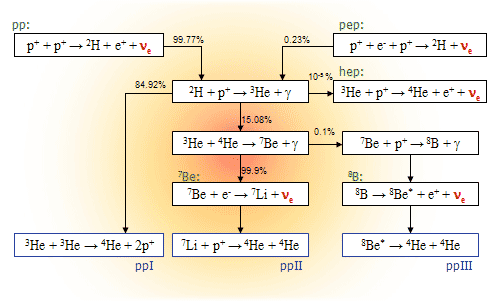
\includegraphics[width=0.99\textwidth]{./images/3nu/solar/pp_chain.png}\\
  \end{column}
  \begin{column}{0.30\textwidth}
   \centering
   {\scriptsize
   This proceeds via the chain reaction shown on the left (pp chain)
   The pp chain dominates for stars up to the Sun's size.
   The primary alternative is the CNO cycle which dominates in stars
   with mass $> M_{sun}$.
   In the Sun the CNO sycle contributes $\sim$1\% of the produced
   energy.\\
   }
  \end{column}
\end{columns}
\end{frame}


\begin{frame}[t]{Solar neutrino flux}
\centering
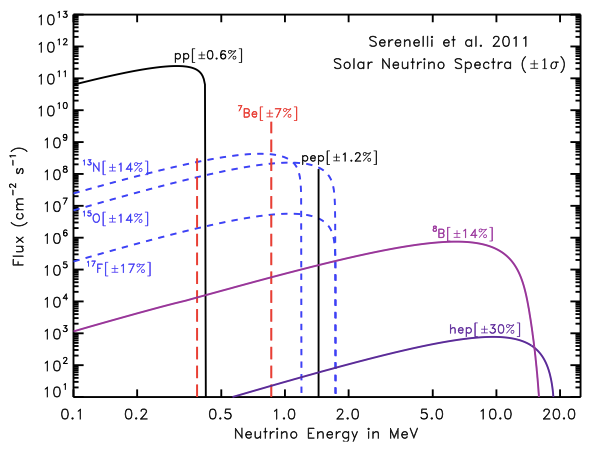
\includegraphics[width=0.85\textwidth]{./images/3nu/solar/solar_nu_flux_2.png}\\
\end{frame}

\begin{frame}[t]{Detection of solar neutrinos: Homestake experiment}

The Davis experiment (1969-99): Using 600 tonnes of $C_{2}Cl_{4}$ in vessel deep in the Homestake mine
($\sim$ 1.5 km) to shield the experiment from cosmic backgrounds.\\
\vspace{0.3cm}
\begin{columns}
  \begin{column}{0.45\textwidth}
    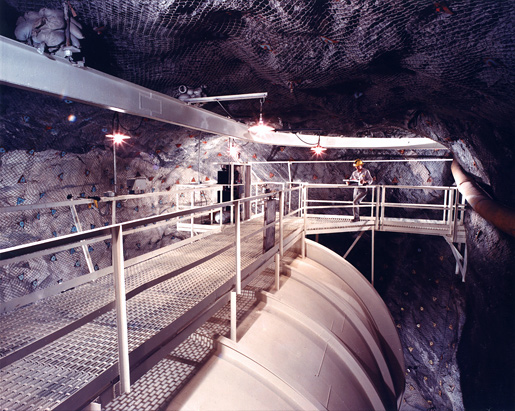
\includegraphics[width=0.98\textwidth]{./images/3nu/solar/davis_experiment_photo.png}\\
  \end{column}
  \begin{column}{0.55\textwidth}
    \begin{itemize}
    {\small
     \item Detection: {\color{red}$\nu_{e} + ^{37}Cl \rightarrow e^{-}
         + ^{37}Ar$}\\
     \item Energy threshold: 814 keV
    \begin{itemize}
     {\small
        \item Sensitive to the $^{8}B$
          and $^{7}Be$ neutrinos of the pp chain
    }
    \end{itemize}
     \item Extract the $^{37}Ar$ ($\sim$monthly) and
       count the number of $^{37}Ar$ atoms
      \begin{itemize}
       {\small
         \item Using the EC reaction: {\color{red}$^{37}Ar +
           e^{-} \rightarrow ^{37}Cl + \nu_{e}$}
         \item $\tau_{1/2}$ = 35 days
         \item Produces a 2.82 keV Auger $e^{-}$
       }
       \end{itemize}
    }
    \end{itemize}
  \end{column}
\end{columns}
\end{frame}

\begin{frame}[t]{Homestake results}

\begin{center}
Solar Standard Model (SSM) prediction for Homestake:  {\color{blue}8.5 $\pm$ 1.8 SNU}\\
(1 SNU = $10^{-36}$ interactions per target atom per sec.)\\
\end{center}
\vspace{0.4cm}
\begin{columns}
  \begin{column}{0.67\textwidth}
     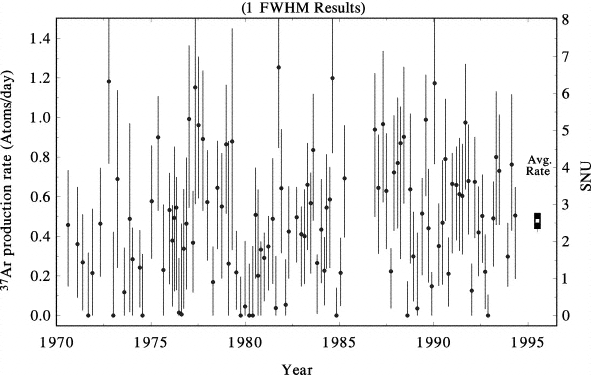
\includegraphics[width=0.95\textwidth]{./images/3nu/solar/homestake_results.png}\\
  \end{column}
  \begin{column}{0.33\textwidth}
   \begin{center}
      Measured a flux of:\\ {\color{red}2.56 $\pm$ 0.23 SNU}\\
      {\small ($\sim$1 $^{37}Ar$ atom /2 days!)}\\
      \vspace{0.4cm}
      {\color{red}$\sim$30\%} of the prediction!.\\
      \vspace{0.4cm}
      That deficit became known as the\\ {\color{red} `solar neutrino problem'}
   \end{center}
  \end{column}
\end{columns}
\end{frame}


\begin{frame}[t]{What was wrong??}

\begin{itemize}
  \item {\color{red} The experiment must be wrong}
  \begin{itemize}
     \item How confident are we in the knowledge of the efficiency extracting a dozen
       of $^{37}Ar$ atoms out of $\sim$600 tonnes of cleaning fluid?
  \end{itemize}
  \item {\color{red} Or the theory must be wrong}
  \begin{itemize}
     \item The predicted flux has strong temperature dependence ($\Phi_{\nu} \propto T^{m}$)
        \begin{itemize}
           \item For pp neutrinos, m=-1.1
           \item ... but for $^{7}Be$ neutrinos, m=+10 (!)
           \item ... and for $^{8}B$ neutrinos, m=+24 (!!)
        \end{itemize}
     \item A small change in temperature could change the $^{7}Be$ and $^{8}B$ flux significantly
  \end{itemize}
  \item {\color{blue} Or something must be wrong with the neutrino?}
\end{itemize}
\end{frame}


\begin{frame}[t]{Solar neutrino detection by GALLEX/GNO and SAGE}

\begin{center}
{\bf Reducing the dependence on the SSM: Measure pp neutrinos.}\\
\end{center}
\begin{columns}
  \begin{column}{0.55\textwidth}
    \centering
     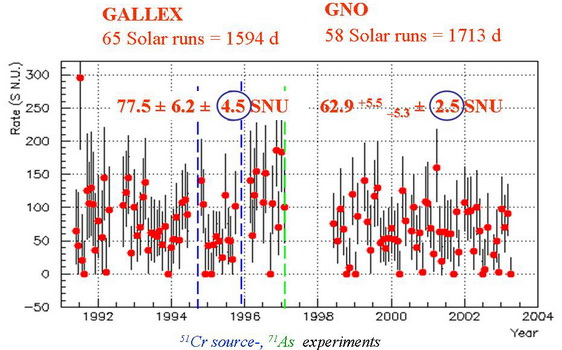
\includegraphics[width=0.95\textwidth]{./images/3nu/solar/gallex_gno_results.jpg}\\
     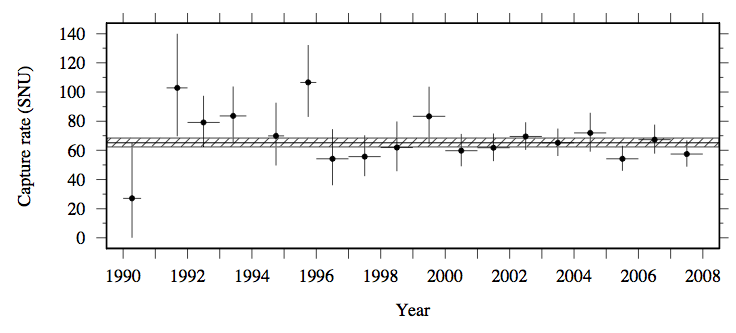
\includegraphics[width=0.90\textwidth]{./images/3nu/solar/sage_results.png}\\
  \end{column}
  \begin{column}{0.45\textwidth}
    \begin{itemize}
    {\small
      \item New generation of Gallium radiochemical experiments
      \item Detection: {\color{red}$\nu_{e} + ^{71}Ga \rightarrow e^{-} + ^{71}Ge$}
      \item Threshold: 233 keV
        \begin{itemize}
        {\small
            \item  sensitive to pp
        }
        \end{itemize}
      \item 130 SNU ($\pm$12) predicted.
      \item Seeing around 50\% of that.\\
    }
    \end{itemize}
      {\scriptsize
         \color{blue}
           [GALLEX: Phys.Lett.B 685 (2010) 47; GNO: Phys.Lett. B 616
           (2005) 174; SAGE: Phys.Rev. C80 (2009) 015807]
      }
  \end{column}
\end{columns}
\end{frame}


\begin{frame}[t]{Solar neutrino detection by (Super-)Kamiokande}

\begin{columns}
  \begin{column}{0.40\textwidth}
     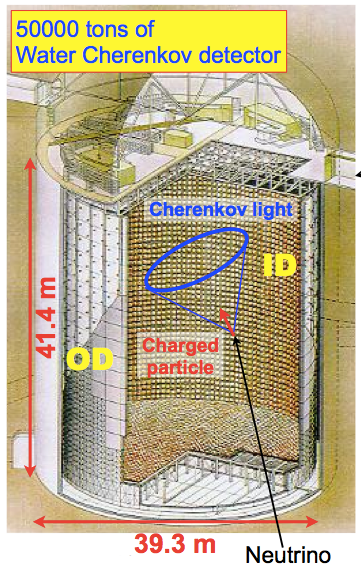
\includegraphics[width=0.95\textwidth]{./images/3nu/solar/sk_schematic.png}\\
     {\scriptsize \color{blue}[Y.Koshio, Neutrino 2014, Boston]}
  \end{column}
  \begin{column}{0.30\textwidth}
     {\scriptsize
      {\bf Kamiokande} (3 kt):\\
         1983-96, 3 phases
      {\bf Super-Kamiokande} (50 kt):\\
         1996-now, 4 phases\\
         \vspace{0.1cm}
     }
     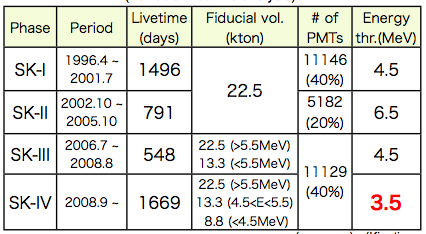
\includegraphics[width=0.99\textwidth]{./images/3nu/solar/sk_phases_and_solar_exposure.png}\\
     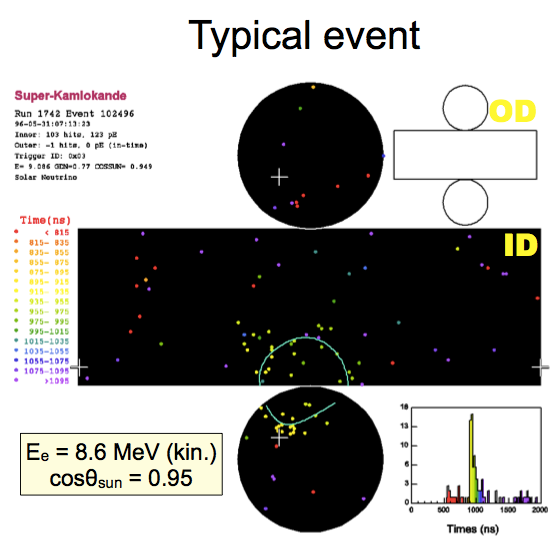
\includegraphics[width=0.99\textwidth]{./images/3nu/solar/sk_solar_event.png}\\
  \end{column}
  \begin{column}{0.30\textwidth}
    {\scriptsize
     Detection via $\nu+e^{-}$ elastic scattering: {\color{red}$\nu+e^{-} \rightarrow \nu+e^{-}$}\\
     \vspace{0.2cm}
     Energy threshold: $\sim$5 MeV.\\
     Sensitive to the $^{8}B$ neutrino flux component.
     \vspace{0.2cm}
     \begin{itemize}
       \item Timing:\\
          Day/night asymmetry and seasonal variations
       \item Directionality
       \item Energy spectrum
     \end{itemize}
     \vspace{0.2cm}
     SK-IV performance:\\
     \begin{itemize}
       \item 55 cm vertex resolution
       \item 23 degrees angular resolution
       \item 14\% energy resolution
     \end{itemize}
    }
  \end{column}
\end{columns}
\end{frame}

\begin{frame}[t]{Solar neutrino detection by (Super-)Kamiokande}

\begin{columns}
  \begin{column}{0.52\textwidth}
    Initial Kamiokande result (1989):\\
     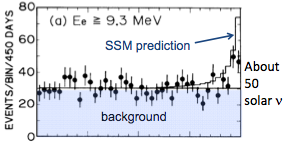
\includegraphics[width=0.95\textwidth]{./images/3nu/solar/kamiokande_solar_costheta.png}\\
    \vspace{0.1cm}
    \begin{itemize}
       \item Strong forward peak
       \begin{itemize}
         \item Direct evidence of neutrino production at the solar core
       \end{itemize}
       \item Observed deficit
       \begin{itemize}
         \item 0.46 $\pm$ 0.13(stat) $\pm$ 0.08(syst) of SSM prediction.\\
       \end{itemize}
    \end{itemize}
    \begin{center}
      {\scriptsize \color{blue}[PRL 63, 16 (1989)]\\}
    \end{center}
  \end{column}
  \begin{column}{0.48\textwidth}
     Latest Super-Kamiokande result:\\
     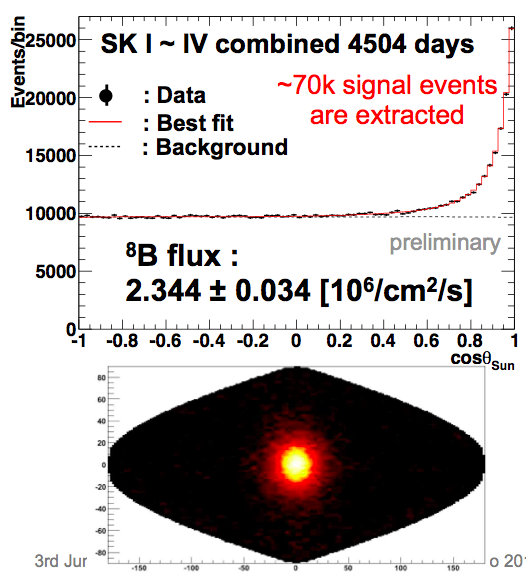
\includegraphics[width=0.95\textwidth]{./images/3nu/solar/sk_solar_costheta_2014.png}\\
     \begin{center}
       {\scriptsize \color{blue}[Y.Koshio, Neutrino 2014, Boston]\\}
     \end{center}
  \end{column}
\end{columns}
\end{frame}


\begin{frame}[t]{Solar neutrino problem - Observed deficits (circa 2000)}

\begin{center}
  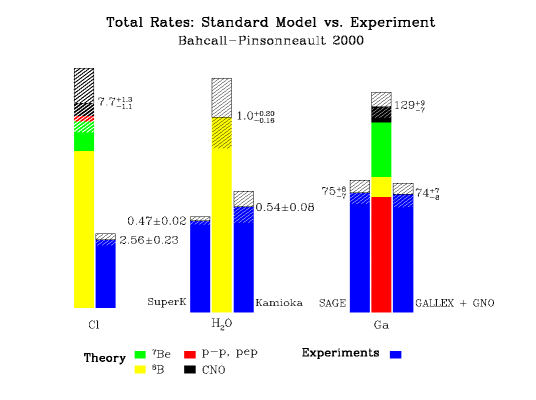
\includegraphics[width=0.90\textwidth]{./images/3nu/solar/colortheoryvsexp2000.png}\\
\end{center}
\end{frame}


\begin{frame}[t]{Solving the solar neutrino problem}

\begin{columns}
  \begin{column}{0.35\textwidth}
    \centering
     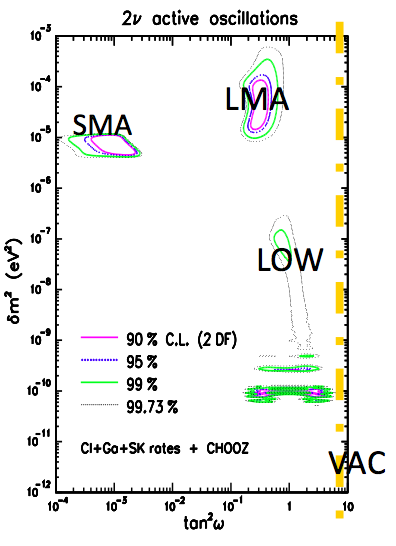
\includegraphics[width=0.99\textwidth]{./images/3nu/solar/contours_pre_sno.png}\\
     \vspace{0.1cm}
     {\scriptsize
     {\color{red}But no smoking-gun signature.}\\
     Solar data fits preferred the Large Mixing Angle (LMA) solution,
     but other regions could not be ruled out.\\
     }
  \end{column}
  \begin{column}{0.65\textwidth}
   {\small
     A heavy water experiment was proposed, able to {\bf measure both} the:
     \begin{itemize}
       \item {\bf CC rate} ($\nu_{e}$ flux), and
       \item {\bf NC rate} ($\nu_{e}$+$\nu_{\mu}$+$\nu_{\tau}$ flux)
     \end{itemize}
     and establish conclusively ({\color{red}independently of solar model calculations})
     the existence of solar neutrino flavour oscillations.\\
     }
     \vspace{0.3cm}
     {
       \centering
       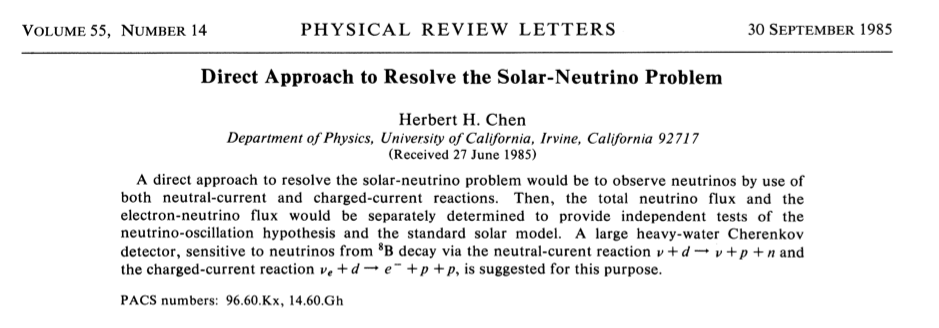
\includegraphics[width=0.99\textwidth]{./images/3nu/solar/chen_prl_abstract.png}\\
       {\scriptsize \color{blue}[H.Chen, Phys.Rev.Lett. 55 (1985) 1534]}\\
     }
  \end{column}
\end{columns}
\end{frame}

\begin{frame}[t]{The SNO experiment}

{\small
SNO (Sudbury Neutrino Observatory) located 2km underground
at the Sudbury nickel mine in Canada:
1,000 tonnes of heavy water in acrylic vessel of 6 m radius,
surrounded by 6,500 tonnes of normal water.
Instrumented with 9,438 photomultipliers (54\% photocathode coverage).
}
\begin{columns}
  \begin{column}{0.50\textwidth}
     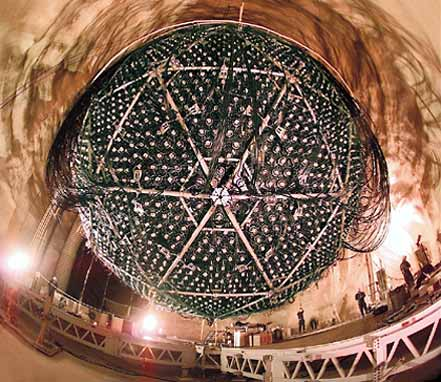
\includegraphics[width=0.95\textwidth]{./images/3nu/solar/sno_detector_photo.jpg}\\
  \end{column}
  \begin{column}{0.50\textwidth}
     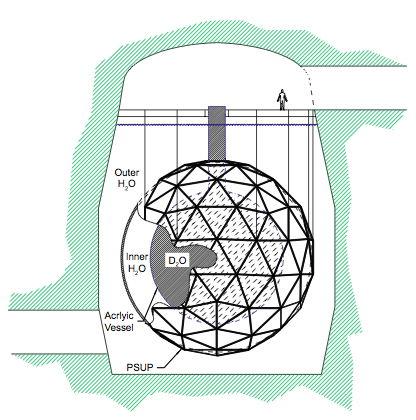
\includegraphics[width=0.95\textwidth]{./images/3nu/solar/sno_detector_schematic.png}\\
  \end{column}
\end{columns}
\end{frame}

\begin{frame}[t]{The SNO experiment - Neutrino detection mechanisms}

%SNO detected solar neutrinos through a variety of mechanicms:
\begin{itemize}
  \item CC ({\color{red}$\nu_{e}+d \rightarrow e^{-}+p+p$}) -1.44 MeV
     \begin{itemize}
          \item Sensitive only to $\nu_{e}$
     \end{itemize}
  \item NC ({\color{blue}$\nu+d \rightarrow \nu+p+n$}) -2.22 MeV
     \begin{itemize}
          \item {\bf Phase 1} (Nov 99 - May 01): {\bf Pure heavy water}\\
                   \begin{itemize}
                      \item Neutrons detected via {\color{orange}n+d $\rightarrow$ t+$\gamma$} (6.3 MeV),
                            $\sigma$ = 0.52 mb
                      \item Using the Cherenkov light of $e^{-}$ from the Compton scattering of $\gamma$
                   \end{itemize}
          \item {\bf Phase 2} (Jul 01 - Sep 03): {\bf Salt phase} (2 tonnes of NaCl)\\
                   \begin{itemize}
                      \item Neutrons detected via
                            {\color{orange}n+$^{35}Cl$ $\rightarrow$ $^{36}Cl+\gamma's$} (8.6 MeV),
                            $\sigma$ = 0.44 b
%                     \item Higher capture efficiency.
                   \end{itemize}
          \item {\bf Phase 3} (Nov 04 - Nov 06): {\bf NCD phase} (36 $^{3}$He proport. counters)\\
                   \begin{itemize}
                      \item Neutrons detected directly via
                            {\color{orange}n+$^{3}He$ $\rightarrow$ p+t}, $\sigma$=5333 barns
                      \item No statistical separation, breaks correlations with CC rate measurement
                   \end{itemize}
     \end{itemize}
  \item $\nu+e^{-}$ elastic ({\color{green} $\nu+e^{-} \rightarrow \nu+e^{-} $}) $\leftarrow$ As in Super-K
     \begin{itemize}
          \item Sensitive to all neutrino flavours
          \item Cross-section for $\nu_{e}$ about 6 times larger than that of  $\nu_{\mu}$ or  $\nu_{\tau}$.
     \end{itemize}
\end{itemize}
Backgrounds mainly from the radioactive decay chains of U and Th
\end{frame}


\begin{frame}[t]{The SNO results}

\begin{columns}
  \begin{column}{0.35\textwidth}
     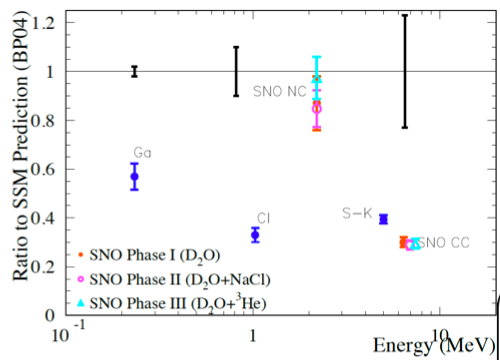
\includegraphics[width=0.99\textwidth]{./images/3nu/solar/sno_results.png}\\
     \begin{itemize}
     {\scriptsize
       \item Total $\nu$ flux from NC rate in agreement with SSM for $^{8}B$ $\nu$'s
             ($\Phi_{SSM}$=(5.05 +1.01 -0.81) $\times$ 10$^{6}$ cm$^{-2}$ s$^{-1}$)
       \item $\nu_{e}$ flux from CC rate much smaller (oscillations!)
       \item Flux from ES rate larger than flux from CC (some contributions from ($\nu_{\mu}$+$\nu_{\tau}$)
             and consistent with SuperK.\\
     }
     \end{itemize}
  \end{column}
  \begin{column}{0.65\textwidth}
     {\scriptsize
       {\color{red}
         $\Phi^{CC}_{SNO}$ = (1.76 $\pm$ 0.06 (stat) $\pm$ 0.09 (syst))
            $\times$ 10$^{6}$ cm$^{-2}$ s$^{-1}$\\
       }
       {\color{blue}
         $\Phi^{NC}_{SNO}$ = (5.09 $\pm$ 0.44 (stat) $\pm$ 0.46 (syst))
            $\times$ 10$^{6}$ cm$^{-2}$ s$^{-1}$\\
       }
       {\color{green}
         $\Phi^{ES}_{SNO}$ = (2.39 $\pm$ 0.24 (stat) $\pm$ 0.12 (syst))
            $\times$ 10$^{6}$ cm$^{-2}$ s$^{-1}$\\
       }
     }
     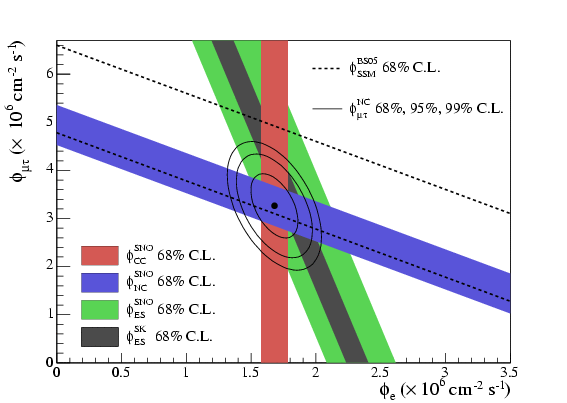
\includegraphics[width=0.99\textwidth]{./images/3nu/solar/sno_results_4lines_nolabels.png}\\
  \end{column}
\end{columns}
{\tiny
 Phase 1: {\color{blue} [PRL 87 (2001) 071301; PRL 89 (2002) 011301; PRL 89 (2002) 011302; PRC 75 (2007) 045502]},
 Phase 2: {\color{blue} [PRL 92 (2004) 181301; PRC 72 (2005) 055502]},
 Phase 3: {\color{blue} [PRL 101 (2008) 111301]},
 Combined:{\color{blue} [PRC 88 (2013) 025501]}\\
}
\end{frame}


\begin{frame}[t]{Explanation of solar experiment results}

\begin{center}
{\bf The solar results favour the {\color{red}large mixing angle MSW solution}.}\\
(with $\theta_{12} \approx$ 33$^{o}$ and ${\Delta}m^{2}_{21} \approx 5\times 10^{-5}$ $eV^{2}/c^{4}$)\\
\end{center}
\begin{block}{}
{\small
\centering
You must have seen at your theory lectures that due to coherent forward scattering, $\nu_{e}$'s propagating in
matter feel a potential that $\nu_{\mu}$'s and $\nu_{\tau}$'s do not.\\
\vspace{0.2cm}
The oscillation probability is modified by matter effects ($x = \frac{2\sqrt{2}G_{F}N_{e}E}{{\Delta}m^{2}}$):
\[
  \displaystyle
%  sin^{2}2{\bf \color{red}\theta_{m}} = \frac{sin^{2}2\theta}{sin^{2}2\theta + (cos2\theta-x)^{2}},\;
  sin2{\bf \color{red}\theta_{m}} = \frac{sin2\theta}{\sqrt{sin^{2}2\theta + (cos2\theta-x)^{2}}},\;
  cos2{\bf \color{red}\theta_{m}} = \frac{cos2\theta-x}{\sqrt{sin^{2}2\theta + (cos2\theta-x)^{2}}}
%  x = \frac{2\sqrt{2}G_{F}N_{e}E}{{\Delta}m^{2}}
\]
{
\scriptsize \color{blue}[Wolfenstein, PRD17 (1978) 2369; Mikheyev and Smirnov, Sov. J. Nucl. Phys. 42 (1985) 913]}
}
\end{block}

\begin{itemize}
{\scriptsize
\item For a neutrino created in the dense solar core $\theta_{m} \rightarrow \pi/2$.
\item If $\theta < \pi/4$ in vacuum, the composition of the weak eigenstates is reversed.
\item $\nu_{e}$ is mostly $\nu_{1}$ in vacuum, but mostly $\nu_{2}$ in the dense solar core.
\item Remains in this state as it travels in regions of lower density (if density changes slowly).\\
}
\end{itemize}

%\item In vacuum $\nu_{e}$ is mostly $\nu_{1}$: {\color{red}$\nu_{e}$ = $cos\theta \cdot \nu_{1}$ + $sin\theta \cdot \nu_{2}$, $\theta < \pi/2$}
% The composition of the weak eigenstates is reversed and $\nu_{e}$ is now mostly $\nu_{2}$.
%Neutrinos are produced in the dense solar core. At high densities there can be no $\nu_{e}$ oscillations
%      ({\color{red}$x \rightarrow \infty$ $\Rightarrow$ $sin^{2}2\theta_{m} \rightarrow$ 0 for any $\theta$})
%\item But as neutrinos propagage towards the Sun's atmosphere they go through regions with the
%      right density for resonance conversion.
%\item The very low energy neutrinos have too low energy for resonant matter oscillation,
%      but oscillate in vaccum (observe the average over several cycles)\\
%\begin{itemize}
%{\scriptsize
%\item Neutrinos are produced in the dense solar core. At high densities there can be no $\nu_{e}$ oscillations
%      ({\color{red}$x \rightarrow \infty$ $\Rightarrow$ $sin^{2}2\theta_{m} \rightarrow$ 0 for any $\theta$})
%\item But as neutrinos propagage towards the Sun's atmosphere they go through regions with the
%      right density for resonance conversion.
%\item The very low energy neutrinos have too low energy for resonant matter oscillation,
%      but oscillate in vaccum (observe the average over several cycles)\\
%}
%\end{itemize}
\end{frame}


\begin{frame}[t]{Confirmation with man-made neutrinos: KamLAND}

\vspace{0.1cm}
\begin{columns}
  \begin{column}{0.30\textwidth}
    \centering
    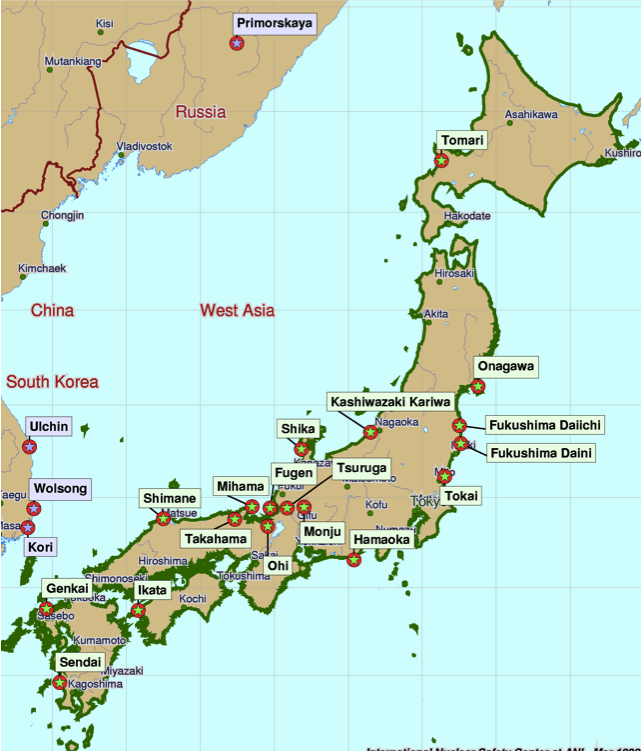
\includegraphics[width=0.99\textwidth]{./images/3nu/reactor/kamLAND_reactors.png}\\
    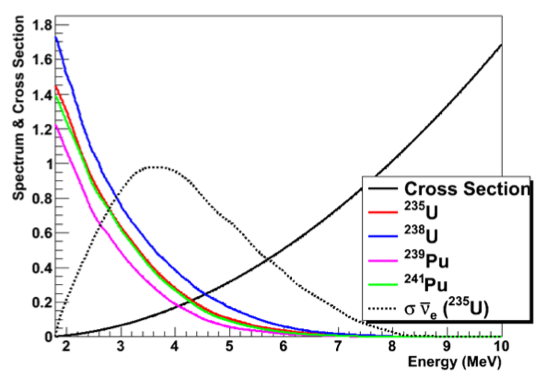
\includegraphics[width=0.99\textwidth]{./images/3nu/reactor/reactor_flux_xsec_and_rate.png}\\
    {\scriptsize \color{blue}[plot from Qian and Wang, arXiv:1405.7217]}
  \end{column}
  \begin{column}{0.70\textwidth}
    \begin{itemize}
    {\small
      \item {\bf Using neutrinos from nuclear reactors}
        \begin{itemize}
        {\scriptsize
           \item 68 $GW_{th}$ of nuclear power (20\% of the world's nuclear power) were available before the Tohoku earthquake.
           \item $\sim$80\% within 140-210 km from the Kamioka mine ($<L>$ $\sim$ 180 km)
        }
        \end{itemize}
      \item {\bf Reactors are sources of a pure and isotropic flux of $\bar{\nu}_{e}$}
        \begin{itemize}
        {\scriptsize
            \item On average, 6 $\bar{\nu}_{e}$ per fission along the decay chain of all fission products.
            \item A 1 $GW_{th}$ reactor emits 2 $\times10^{20}$ $\bar{\nu}_{e}$ /sec.
            \item Main $\bar{\nu}_{e}$ sources: $^{235}U$, $^{238}U$, $^{239}Pu$, $^{241}Pu$.
        }
        \end{itemize}
      \item {\bf $\bar{\nu}_{e}$ detection:}
        \begin{itemize}
        {\scriptsize
            \item Prompt $e^{+}$ signal
                  ({\color{red}$\bar{\nu}_{e}$ + p $\rightarrow$ $e^{+}$ + n})
            \item Followed (within 200 $\mu$s) by a correlated signal from neutron capture
                  ({\color{red}n + p $\rightarrow$ d + $\gamma$} (2.2 eV))
        }
        \end{itemize}
      \item {\bf $\bar{\nu}_{e}$ energy reconstruction:} $E_{\nu} = T_{e} + 1.8 MeV$
    }
    \end{itemize}
  \end{column}
\end{columns}
\end{frame}


\begin{frame}[t]{The KamLAND experiment}

\begin{columns}
  \begin{column}{0.50\textwidth}
   \centering
     \includegraphics[width=0.95\textwidth]{./images/3nu/reactor/kamLAND_schematic.png}\\
     \vspace{0.3cm}
     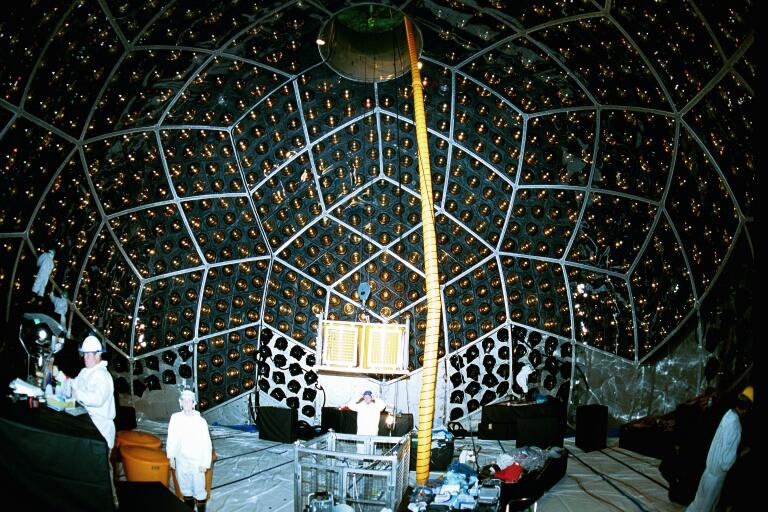
\includegraphics[width=0.75\textwidth]{./images/3nu/reactor/kamLAND_interior_photo.jpg}\\
  \end{column}
  \begin{column}{0.50\textwidth}
     Detector:
     \begin{itemize}
         \item 1,000 tonnes of liquid scintillator in a 13 m diameter nylon balloon
         \item Within 18 m diameter stainless steel vessel, filled with mineral oil to shield the target
               region from external radiation
         \item Viewed by 1879 (554 20'' and 1325 17'') photomultipliers
         \item Surrounded by Water Cherenkov detector to absorb $\gamma$, n and tag cosmic $\mu$
         \item In 2700 m.w.e depth
     \end{itemize}
  \end{column}
\end{columns}
\end{frame}



\begin{frame}[t]{KamLAND results}

{\small \bf \centering
KamLAND saw $\bar{\nu}_{e}$ disappearance and energy spectrum distortion ($>$5$\sigma$).\\
}
\vspace{0.3cm}
\begin{columns}
  \begin{column}{0.40\textwidth}
     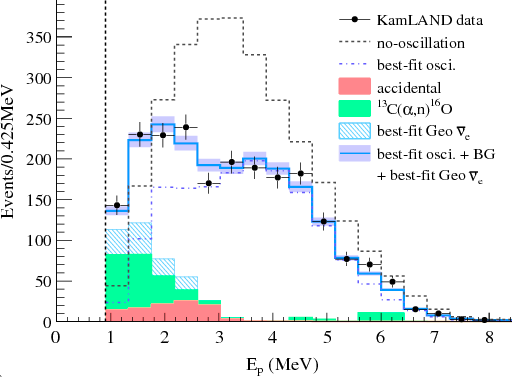
\includegraphics[width=0.95\textwidth]{./images/3nu/reactor/kamLAND_energy_spectrum_noeff.png}\\
     {\scriptsize
     Backgrounds:\\
     \begin{itemize}
        \item Accidental
        \item Terrestrial neutrinos (from $^{238}$U and $^{232}$Th in the Earth crust and mantle)
        \item {\bf Correlated}: Fast neutrons, $\alpha$ decays $^{13}$C($\alpha$,n)$^{16}O$* and
              $^{9}Li$ and $^{8}He$ spallation products
     \end{itemize}
     }
  \end{column}
  \begin{column}{0.60\textwidth}
    \centering
     {\small \color{red}Smoking-gun signature for neutrino oscillations!}\\
     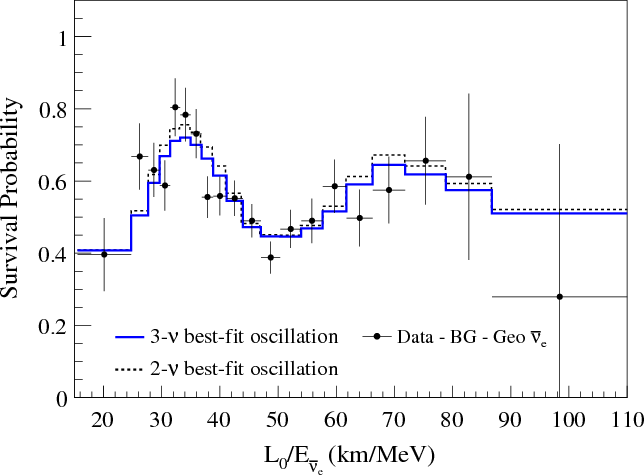
\includegraphics[width=0.99\textwidth]{./images/3nu/reactor/kamLAND_oscillations.png}\\
     {\scriptsize \color{blue}[Abe et al., Phys.Rev.Lett. 100 (2008) 221803]}
  \end{column}
\end{columns}
\end{frame}


\begin{frame}[t]{Oscillation analysis of KamLAND+solar results}

\centering
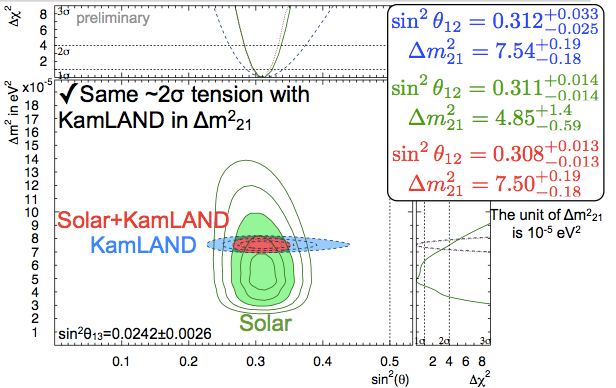
\includegraphics[width=0.95\textwidth]{./images/3nu/solar/global_osc_results.png}\\
\end{frame}

\begin{frame}[t]{Future prospects: Probing the transition region}

\begin{columns}
  \begin{column}{0.70\textwidth}
      Precision oscillation measurements and a probe of the {\color{red} transition region} to
      \begin{itemize}
         \item confirm MSW and
         \item search for non-standard neutrino physics.
      \end{itemize}
  \end{column}
  \begin{column}{0.30\textwidth}
      \begin{block}{}
      {\scriptsize
       \centering
         Measuring low energy \\ solar neurinos is also\\ important in order to\\ improve the SSM model.\\
      }
      \end{block}
  \end{column}
\end{columns}
\begin{center}
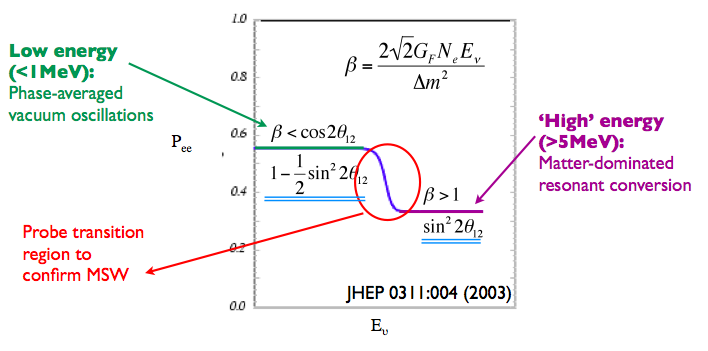
\includegraphics[width=0.80\textwidth]{./images/3nu/solar/Pee.png}\\
{\scriptsize \color{blue}[schematic by O.Gann, Neutrino 2014 conference, Boston]}
\end{center}
\end{frame}

%
%
%

\begin{frame}[t]{Future prospects: Confirming MSW}

\begin{columns}
  \begin{column}{0.65\textwidth}
    \centering
     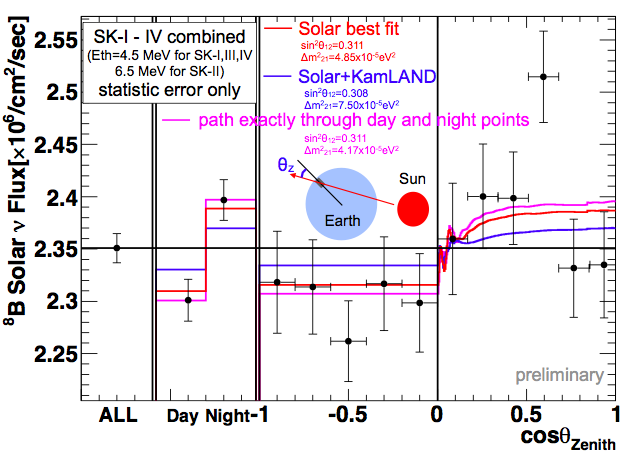
\includegraphics[width=0.95\textwidth]{./images/3nu/solar/sk_day_night_zenith.png}\\
     \vspace{0.2cm}
     {\color{blue}[Phys.Rev.Lett. 112 (2014) 091805]}
  \end{column}
  \begin{column}{0.35\textwidth}
     \begin{center}
     {\scriptsize
       {\bf Direct test of matter effects.}\\
       \vspace{0.2cm}
       Day-night difference in the solar neutrino flux.\\
       \vspace{0.2cm}
       Super-K observes the difference between the average day and night rates
       over the average of the two rates to be:\\
       \vspace{0.2cm}
       {\color{red}(-3.2 $\pm$1.1 (stat) $\pm$0.5(syst))\%}\\
       \vspace{0.2cm}
       which deviates from 0 by 2.7$\sigma$\\
     }
     \end{center}
  \end{column}
\end{columns}
\end{frame}

%
%
%

\begin{frame}[t]{Borexino experiment - Neutrino spectroscopy}

 \vspace{-0.3cm}
 {\small
 Large volume radio-pure {\bf liquid scintillator detector} (2007-present).\\
 Located deep underground (3,800 m.w.e.) in the hall C of Gran Sasso laboratory.
 }
 \vspace{-0.5cm}
  \begin{columns}[T]
    \begin{column}{0.47\textwidth}
      \begin{center}
       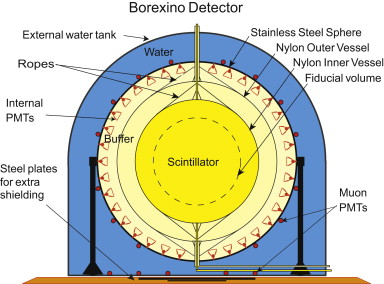
\includegraphics[width=0.80\textwidth]{./images/3nu/solar/borexino_schematic}\\
       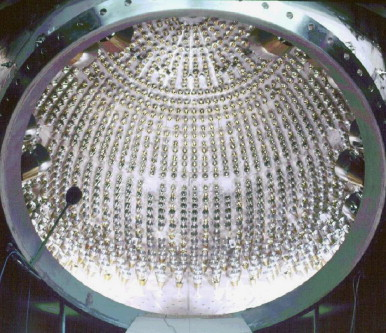
\includegraphics[width=0.60\textwidth]{./images/3nu/solar/borexino_stainless_steel}\\
      \end{center}
    \end{column}
    \begin{column}{0.53\textwidth}
        \begin{center}
         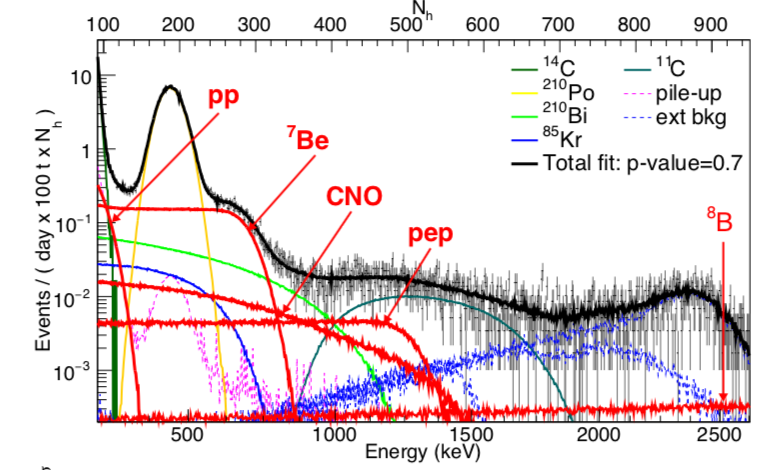
\includegraphics[width=0.80\textwidth]{./images/3nu/solar/borexino_spectroscopy_1}\\
         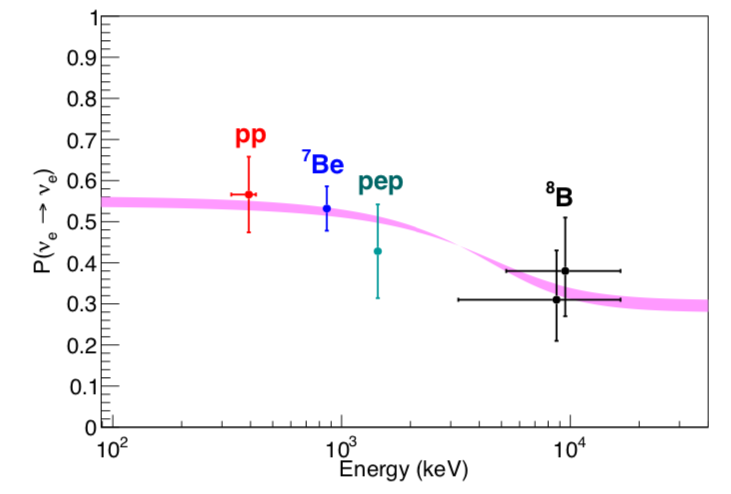
\includegraphics[width=0.60\textwidth]{./images/3nu/solar/borexino_spectroscopy_2}\\
         {\scriptsize \color{blue}[M.Agostini et al., arXiv:1707.09279]}
        \end{center}
    \end{column}
  \end{columns}

\end{frame}

%
%
%

\begin{frame}[t]{Future prospects: Probing the transition region}

\begin{columns}
  \begin{column}{0.22\textwidth}
     \centering
     {\bf Sterile $\nu$}\\
     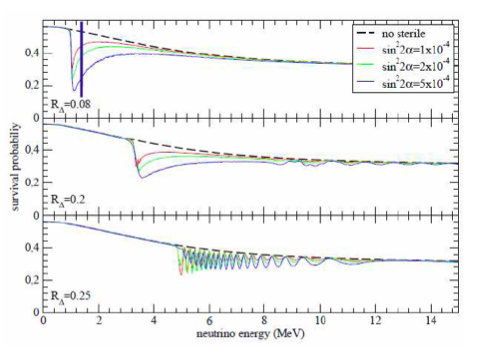
\includegraphics[width=0.98\textwidth,height=0.32\textheight]{./images/3nu/solar/solar_nonstd_sterile.png}\\
     {\tiny{\color{blue}[Phys.Rev.D 83 (2011)]}}\\
     {\bf FCNC}\\
     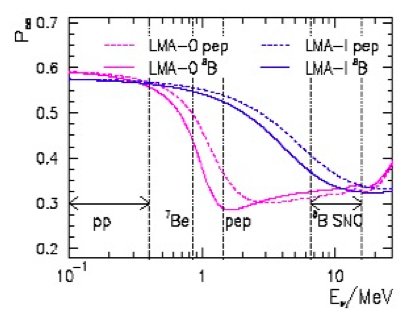
\includegraphics[width=0.98\textwidth,height=0.32\textheight]{./images/3nu/solar/solar_nonstd_fcnc.png}\\
     {\tiny{\color{blue}[Phys.Lett.B 594 (2004)]}}
  \end{column}
  \begin{column}{0.22\textwidth}
     \centering
     {\bf Mass-varying $\nu$}\\
     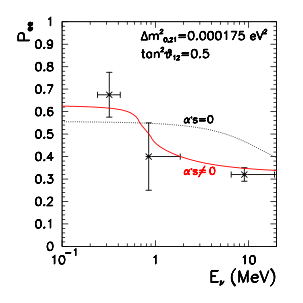
\includegraphics[width=0.98\textwidth,height=0.32\textheight]{./images/3nu/solar/solar_nonstd_mvarying.png}\\
     {\tiny{\color{blue}[Phys.Rept. 460 (2008) 1-129]}}\\
     \vspace{0.8cm}
     {\scriptsize \color{blue}[Plots from O.Gann, Neutrino 2014 conference, Boston]}
  \end{column}
  \begin{column}{0.56\textwidth}
     \centering
      {\bf The transition region provides a sensitive probe of new physics}\\
      \vspace{0.2cm}
     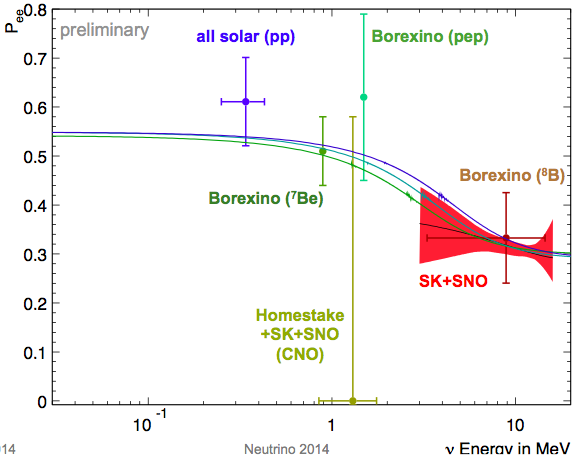
\includegraphics[width=0.95\textwidth]{./images/3nu/solar/Pee_with_data.png}\\
      {\scriptsize \color{blue}[Y.Koshio, Neutrino 2014, Boston]}
  \end{column}
\end{columns}
\begin{center}
\end{center}
\end{frame}




% %
% % What you should know
% %
%
% \begin{frame}{What you should know}
%
% \end{frame}


%
% What to read
%

% \begin{frame}{What to read}
%
% {\color{magenta} Add in next revision}

% MSW effect
% \begin{itemize}
% {\scriptsize
% \item
%   L. Wolfenstein,
%   Neutrino Oscillations in Matter,
%   Phys.Rev. D17 (1978) 2369-2374
%   {\color{magenta}[Wolfenstein:1977ue]}
% }
% \end{itemize}
%
% KamLAND experiment
% \begin{itemize}
% {\scriptsize
% \item
%   KamLAND Collaboration (S. Abe et al.),
%   Precision Measurement of Neutrino Oscillation Parameters with KamLAND,
%   Phys.Rev.Lett. 100 (2008) 221803
%   {\color{magenta}[Abe:2008aa]}
% }
% \end{itemize}

% \end{frame}
